\documentclass{standalone}
\usepackage{tikz}
\usetikzlibrary{patterns, positioning}


\begin{document}
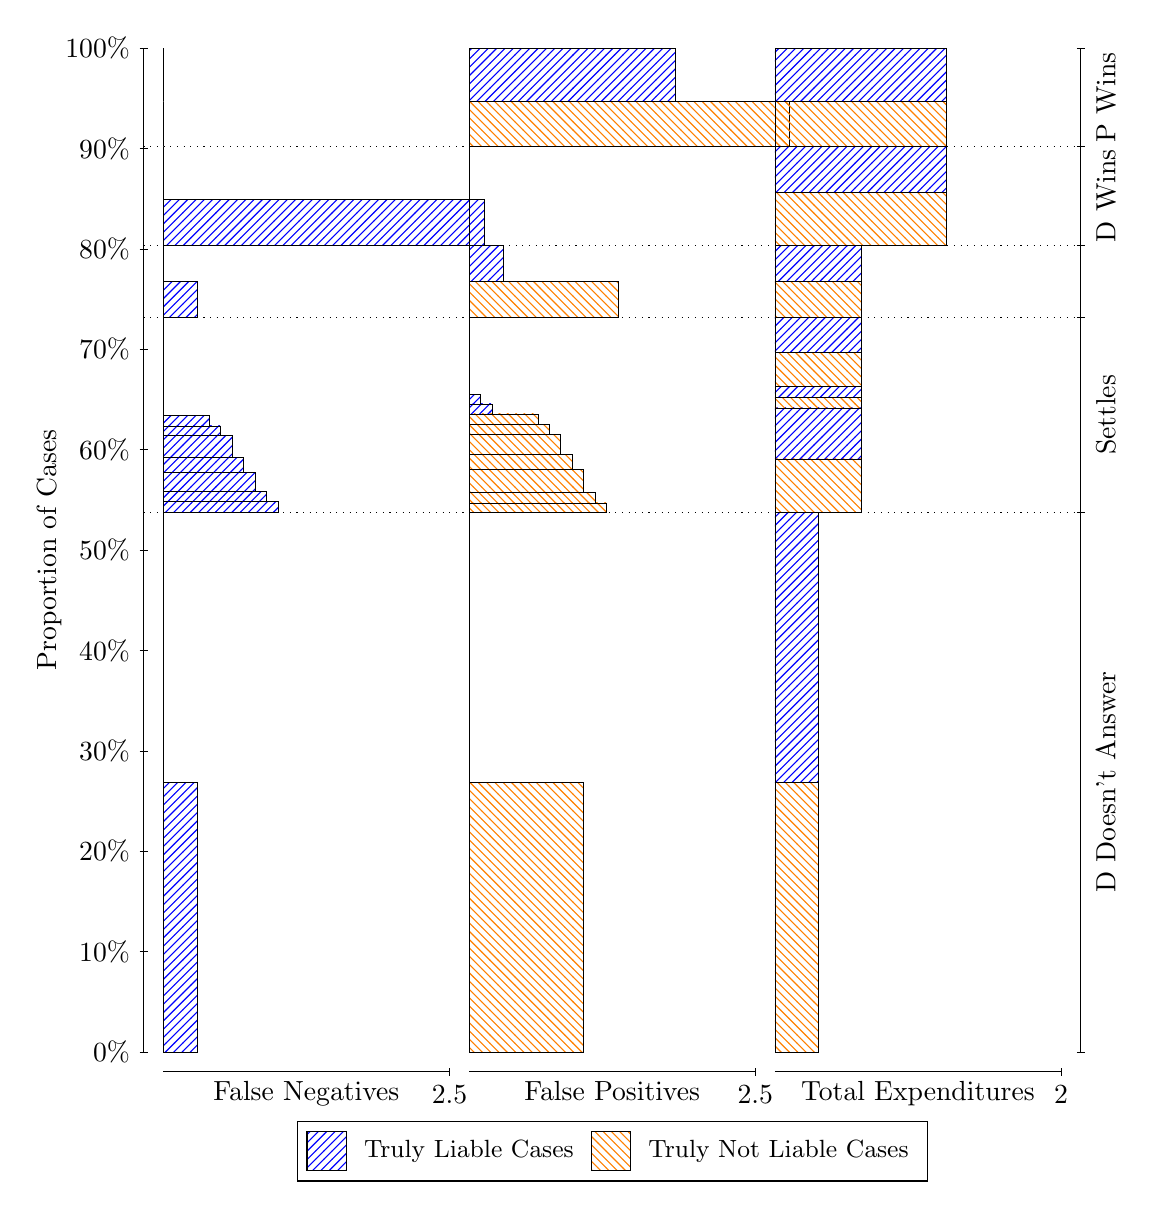
\begin{tikzpicture}
\draw[black, very thin] (1.5,1.75) -- (1.5,14.5);
\node[rotate=90, text=black, anchor=center] at (0.3, 8.125) {Proportion of Cases};
\draw[black, very thin] (1.45,1.75) -- (1.55,1.75);
\node[text=black, anchor=east] at (1.45, 1.75) {0\%};
\draw[black, very thin] (1.45,3.025) -- (1.55,3.025);
\node[text=black, anchor=east] at (1.45, 3.025) {10\%};
\draw[black, very thin] (1.45,4.3) -- (1.55,4.3);
\node[text=black, anchor=east] at (1.45, 4.3) {20\%};
\draw[black, very thin] (1.45,5.575) -- (1.55,5.575);
\node[text=black, anchor=east] at (1.45, 5.575) {30\%};
\draw[black, very thin] (1.45,6.85) -- (1.55,6.85);
\node[text=black, anchor=east] at (1.45, 6.85) {40\%};
\draw[black, very thin] (1.45,8.125) -- (1.55,8.125);
\node[text=black, anchor=east] at (1.45, 8.125) {50\%};
\draw[black, very thin] (1.45,9.4) -- (1.55,9.4);
\node[text=black, anchor=east] at (1.45, 9.4) {60\%};
\draw[black, very thin] (1.45,10.675) -- (1.55,10.675);
\node[text=black, anchor=east] at (1.45, 10.675) {70\%};
\draw[black, very thin] (1.45,11.95) -- (1.55,11.95);
\node[text=black, anchor=east] at (1.45, 11.95) {80\%};
\draw[black, very thin] (1.45,13.225) -- (1.55,13.225);
\node[text=black, anchor=east] at (1.45, 13.225) {90\%};
\draw[black, very thin] (1.45,14.5) -- (1.55,14.5);
\node[text=black, anchor=east] at (1.45, 14.5) {100\%};

\draw[black, very thin] (13.4,1.75) -- (13.4,14.5);
\draw[black, very thin] (13.35,1.75) -- (13.45,1.75);
\node[anchor=west] at (13.35, 1.75) {};
\draw[black, very thin] (13.35,8.6056) -- (13.45,8.6056);
\node[anchor=west] at (13.35, 8.6056) {};
\draw[black, very thin] (13.35,11.077) -- (13.45,11.077);
\node[anchor=west] at (13.35, 11.077) {};
\draw[black, very thin] (13.35,11.997) -- (13.45,11.997);
\node[anchor=west] at (13.35, 11.997) {};
\draw[black, very thin] (13.35,13.247) -- (13.45,13.247);
\node[anchor=west] at (13.35, 13.247) {};
\draw[black, very thin] (13.35,14.5) -- (13.45,14.5);
\node[anchor=west] at (13.35, 14.5) {};

\draw[black, very thin, pattern color=blue, pattern=north east lines] (1.75,1.75) rectangle (2.186,5.1778);
\draw[black, very thin, pattern color=orange, pattern=north west lines] (1.75,5.1778) rectangle (1.75,8.6056);
\draw[black, very thin, pattern color=blue, pattern=north east lines] (1.75,8.6056) rectangle (3.2033,8.7398);
\draw[black, very thin, pattern color=blue, pattern=north east lines] (1.75,8.7398) rectangle (3.058,8.868);
\draw[black, very thin, pattern color=blue, pattern=north east lines] (1.75,8.868) rectangle (2.9127,9.1151);
\draw[black, very thin, pattern color=blue, pattern=north east lines] (1.75,9.1151) rectangle (2.7673,9.301);
\draw[black, very thin, pattern color=blue, pattern=north east lines] (1.75,9.301) rectangle (2.622,9.581);
\draw[black, very thin, pattern color=blue, pattern=north east lines] (1.75,9.581) rectangle (2.4767,9.7015);
\draw[black, very thin, pattern color=blue, pattern=north east lines] (1.75,9.7015) rectangle (2.3313,9.8307);
\draw[black, very thin, pattern color=orange, pattern=north west lines] (1.75,9.8307) rectangle (1.75,11.077);
\draw[black, very thin, pattern color=blue, pattern=north east lines] (1.75,11.077) rectangle (2.186,11.54);
\draw[black, very thin, pattern color=orange, pattern=north west lines] (1.75,11.54) rectangle (1.75,11.997);
\draw[black, very thin, pattern color=blue, pattern=north east lines] (1.75,11.997) rectangle (5.8193,12.575);
\draw[black, very thin, pattern color=orange, pattern=north west lines] (1.75,12.575) rectangle (1.75,13.247);
\draw[black, very thin, pattern color=orange, pattern=north west lines] (1.75,13.247) rectangle (1.75,13.819);
\draw[black, very thin, pattern color=blue, pattern=north east lines] (1.75,13.819) rectangle (1.75,14.5);
\draw[black, very thin, pattern color=orange, pattern=north west lines] (5.6333,1.75) rectangle (7.0867,5.1778);
\draw[black, very thin, pattern color=blue, pattern=north east lines] (5.6333,5.1778) rectangle (5.6333,8.6056);
\draw[black, very thin, pattern color=orange, pattern=north west lines] (5.6333,8.6056) rectangle (7.3773,8.7237);
\draw[black, very thin, pattern color=orange, pattern=north west lines] (5.6333,8.7237) rectangle (7.232,8.8545);
\draw[black, very thin, pattern color=orange, pattern=north west lines] (5.6333,8.8545) rectangle (7.0867,9.153);
\draw[black, very thin, pattern color=orange, pattern=north west lines] (5.6333,9.153) rectangle (6.9413,9.3399);
\draw[black, very thin, pattern color=orange, pattern=north west lines] (5.6333,9.3399) rectangle (6.796,9.5884);
\draw[black, very thin, pattern color=orange, pattern=north west lines] (5.6333,9.5884) rectangle (6.6507,9.7174);
\draw[black, very thin, pattern color=orange, pattern=north west lines] (5.6333,9.7174) rectangle (6.5053,9.8523);
\draw[black, very thin, pattern color=blue, pattern=north east lines] (5.6333,9.8523) rectangle (5.924,9.9815);
\draw[black, very thin, pattern color=blue, pattern=north east lines] (5.6333,9.9815) rectangle (5.7787,10.102);
\draw[black, very thin, pattern color=blue, pattern=north east lines] (5.6333,10.102) rectangle (5.6333,11.077);
\draw[black, very thin, pattern color=orange, pattern=north west lines] (5.6333,11.077) rectangle (7.5227,11.535);
\draw[black, very thin, pattern color=blue, pattern=north east lines] (5.6333,11.535) rectangle (6.0693,11.997);
\draw[black, very thin, pattern color=orange, pattern=north west lines] (5.6333,11.997) rectangle (5.6333,12.669);
\draw[black, very thin, pattern color=blue, pattern=north east lines] (5.6333,12.669) rectangle (5.6333,13.247);
\draw[black, very thin, pattern color=orange, pattern=north west lines] (5.6333,13.247) rectangle (9.7027,13.819);
\draw[black, very thin, pattern color=blue, pattern=north east lines] (5.6333,13.819) rectangle (8.2493,14.5);
\draw[black, very thin, pattern color=orange, pattern=north west lines] (9.5167,1.75) rectangle (10.062,5.1778);
\draw[black, very thin, pattern color=blue, pattern=north east lines] (9.5167,5.1778) rectangle (10.062,8.6056);
\draw[black, very thin, pattern color=orange, pattern=north west lines] (9.5167,8.6056) rectangle (10.607,9.2834);
\draw[black, very thin, pattern color=blue, pattern=north east lines] (9.5167,9.2834) rectangle (10.607,9.931);
\draw[black, very thin, pattern color=orange, pattern=north west lines] (9.5167,9.931) rectangle (10.607,10.066);
\draw[black, very thin, pattern color=blue, pattern=north east lines] (9.5167,10.066) rectangle (10.607,10.2);
\draw[black, very thin, pattern color=orange, pattern=north west lines] (9.5167,10.2) rectangle (10.607,10.634);
\draw[black, very thin, pattern color=blue, pattern=north east lines] (9.5167,10.634) rectangle (10.607,11.077);
\draw[black, very thin, pattern color=orange, pattern=north west lines] (9.5167,11.077) rectangle (10.607,11.535);
\draw[black, very thin, pattern color=blue, pattern=north east lines] (9.5167,11.535) rectangle (10.607,11.997);
\draw[black, very thin, pattern color=orange, pattern=north west lines] (9.5167,11.997) rectangle (11.697,12.669);
\draw[black, very thin, pattern color=blue, pattern=north east lines] (9.5167,12.669) rectangle (11.697,13.247);
\draw[black, very thin, pattern color=orange, pattern=north west lines] (9.5167,13.247) rectangle (11.697,13.819);
\draw[black, very thin, pattern color=blue, pattern=north east lines] (9.5167,13.819) rectangle (11.697,14.5);
\draw[black, dotted] (1.5,8.6056) -- (13.4,8.6056);
\draw[black, dotted] (1.5,11.077) -- (13.4,11.077);
\draw[black, dotted] (1.5,11.997) -- (13.4,11.997);
\draw[black, dotted] (1.5,13.247) -- (13.4,13.247);
\draw[black, very thin] (1.75,1.5) -- (5.3833,1.5);
\node[text=black, anchor=north] at (3.5667, 1.5) {False Negatives};
\draw[black, very thin] (5.3833,1.45) -- (5.3833,1.55);
\node[text=black, anchor=north] at (5.3833, 1.45) {2.5};

\draw[black, very thin] (5.6333,1.5) -- (9.2667,1.5);
\node[text=black, anchor=north] at (7.45, 1.5) {False Positives};
\draw[black, very thin] (9.2667,1.45) -- (9.2667,1.55);
\node[text=black, anchor=north] at (9.2667, 1.45) {2.5};

\draw[black, very thin] (9.5167,1.5) -- (13.15,1.5);
\node[text=black, anchor=north] at (11.333, 1.5) {Total Expenditures};
\draw[black, very thin] (13.15,1.45) -- (13.15,1.55);
\node[text=black, anchor=north] at (13.15, 1.45) {2};

\node[text=black, centered, rotate=90] at (13.72, 5.1778) {D Doesn't Answer};
\node[text=black, centered, rotate=90] at (13.72, 9.8415) {Settles};

\node[text=black, centered, rotate=90] at (13.72, 12.622) {D Wins};
\node[text=black, centered, rotate=90] at (13.72, 13.874) {P Wins};

\draw (7.449999999999999,1.5) node[draw=none] (baseCoordinate) {};
\begin{scope}[align=center]
        \matrix[scale=0.5, draw=black, below=0.5cm of baseCoordinate, nodes={draw}, column sep=0.1cm]{
            \node[rectangle, draw, minimum width=0.5cm, minimum height=0.5cm, pattern color=blue, pattern=north east lines] {}; &
            \node[draw=none, font=\small, text=black] (B) {Truly Liable Cases}; &
            \node[rectangle, draw, minimum width=0.5cm, minimum height=0.5cm, pattern color=orange, pattern=north west lines] {}; &
            \node[draw=none, font=\small, text=black] (B) {Truly Not Liable Cases}; \\
            };
\end{scope}

\end{tikzpicture}
\end{document}